
Robotic workcell has been designed keeping in mind the workspace of handling robot. Handling robot has to able to reach every station in the workspace without any collision. The drawers of storage system is especially close to the production floor and the robot requires
some space to move around without getting stuck. Figure \ref{fig:robotic-workcell} shows the layout of the workcell. The robotic workcell consists of various subsystems which include bending machine, storage station, unloading station, handling robot, bending machine terminal operating robot, safety fence.

% Create a figure of robotic workcell flow of things
\begin{figure}[h]
    \centering
    \begin{tikzpicture}[
        every node/.style={draw, ellipse, align=center, inner sep=5pt, line width=0.4mm},
        rect/.style={draw=cyan, rectangle, rounded corners=8pt, align=center, inner sep=12pt},
        energy/.style={->, >=stealth, thick, line width=0.5mm},
        data/.style={->, >=stealth, dashed, line width=0.5mm},
        material/.style={->, >=stealth, dotted, line width=0.5mm},
        node distance=1cm
    ]
      
        % Nodes
        \node (bending) [red] {\hyperref[sub:bending-machine]{Bending}\\ \hyperref[sub:bending-machine]{Machine}};
        \node (terminal) [red, left=of bending] {\hyperref[sub:bending-machine]{Terminal}};
        \node (camera1) [orange, below left=1cm and 0cm of bending] {\hyperref[sub:bending-machine]{Inspection}\\ \hyperref[sub:bending-machine]{Camera}};
        \node (footpedal) [red, below right=1cm and 0cm of bending] {\hyperref[sub:bending-machine]{Foot}\\ \hyperref[sub:bending-machine]{pedal}};
        \node (plc) [blue, below=4.5cm of bending, inner sep=10pt] {\hyperref[subsec:plc]{PLC}};
        \node (pandarobot) [gray, above left=0.5cm and 1.5cm of plc] {\hyperref[sub:panda-robot]{Panda}\\ \hyperref[sub:panda-robot]{Robot}};
        \node (handlingrobot) [green, above right=0.5cm and 3cm of plc] {\hyperref[sub:handling-robot]{Handling}\\ \hyperref[sub:panda-robot]{Robot}};
        \node (camera3) [green, above right=of handlingrobot] {\hyperref[sub:handling-robot]{Camera}};
        \node (storage) [rect, below=3cm of camera3, text=cyan] {\hyperref[sub:storage-station]{Storage}\\ \hyperref[sub:storage-station]{Station}};
        \node (camera2) [gray, above left=of pandarobot] {\hyperref[sub:panda-robot]{Camera}};
        \node (unloading) [rect, below=of plc, draw=cyan, text=cyan] {\hyperref[sub:unloading-station]{Unloading}\\ \hyperref[sub:unloading-station]{Station}};
        \node (energy) [rectangle, draw=none, fill=white, text width=2.5cm, align=left, above left=0.3cm and 0cm of unloading, font=\footnotesize] {Energy Flow};
        \node (data) [rectangle, draw=none, fill=white, text width=2.5cm, align=left, below=0cm of energy, font=\footnotesize] {Data Flow};
        \node (material) [rectangle, draw=none, fill=white, text width=2.5cm, align=left, below=0cm of data, font=\footnotesize] {Material Flow};
        \node (energy_left) [circle, draw=none, left=0cm of energy] {};
        \node (energy_right) [circle, draw=none, left=1cm of energy_left] {};
        \node (data_left) [circle, draw=none, left=0cm of data] {};
        \node (data_right) [circle, draw=none, left=1cm of data_left] {};
        \node (material_left) [circle, draw=none, left=0cm of material] {};
        \node (material_right) [circle, draw=none, left=1cm of material_left] {};
        
        % Energy flow
        \draw[energy] (bending) -- (terminal);
        \draw[energy] (bending) -- (footpedal);
        \draw[energy, transform canvas={xshift=-4pt}] (plc) -- (camera1);
        \draw[energy] (plc) .. controls ++(-1, 0) and ++(1,-1) .. (pandarobot);
        \draw[energy] (pandarobot) .. controls ++(-1, 0.5) and ++(0.5,-1) .. (camera2);
        \draw[energy] (plc) .. controls ++(1, 0) and ++(-1,-1) .. (handlingrobot);
        \draw[energy] (handlingrobot) .. controls ++(2,1.2) and ++(-2,-1.3) .. (camera3);
        \draw[energy, transform canvas={xshift=-4pt}] (unloading) -- (plc);
        
        % Data flow
        \draw[data] (terminal) .. controls ++(-2,-1) and ++(0,1) .. (camera2);
        \draw[data] (camera2) .. controls ++(1, -0.5) and ++(-1,1) .. (pandarobot);
        \draw[data] (camera3) .. controls ++(-0.5,-1) and ++(2,0.5) .. (handlingrobot);
        \draw[data] (bending) -- (camera1);
        \draw[data] (plc) -- (footpedal);
        \draw[data] (storage) -- (camera3);
        \draw[data] (bending) .. controls ++(5,1) and ++(0,2) .. (camera3);
        \draw[data, transform canvas={xshift=4pt}] (camera1) -- (plc);
        \draw[data, <->, transform canvas={xshift=4pt}] (unloading) -- (plc);
        \draw[data, <->] (plc) .. controls ++(-1, 0.5) and ++(2,-1) .. (pandarobot);
        \draw[data, <->] (plc) .. controls ++(1, 0.4) and ++(-2,-1) .. (handlingrobot);
        \draw[data] (unloading) .. controls ++(8,0) and ++(4,-7) .. (camera3);
        \draw[data] (footpedal) .. controls ++(-0.5,1) and ++(1,-1) .. (bending);

        % Material flow
        \draw[material] (unloading) .. controls ++(2,1) and ++(1,-3) .. (handlingrobot);
        \draw[material] (handlingrobot) .. controls ++(1.5,-0.5) and ++(-1,1) .. (storage);
        \draw[material, <->] (bending) .. controls ++(4,-1) and ++(0,3) .. (handlingrobot);

        % Create legend for the figure
        \draw[energy,-] (energy_left) -- (energy_right);
        \draw[data,-] (data_left) -- (data_right);
        \draw[material,-] (material_left) -- (material_right);

    \end{tikzpicture}
    \caption{Energy, data and material flow in the robotic workcell}
    \label{fig:flow-workcell}
\end{figure}


The preliminary designs for the mobile robot unit were further elaborated
in the form of CAD models and successively converted into final CAD designs. Figure 1 shows the
current status of the mobile robot unit. This consists of several subsystems: the storage box, the robot
unit, the removal station, the VisCheck operating unit and the safety fence. The latter is still in the
preliminary design phase. The other subsystems are described in more detail in the following
subsections.

\begin{figure}[h]
    \centering
    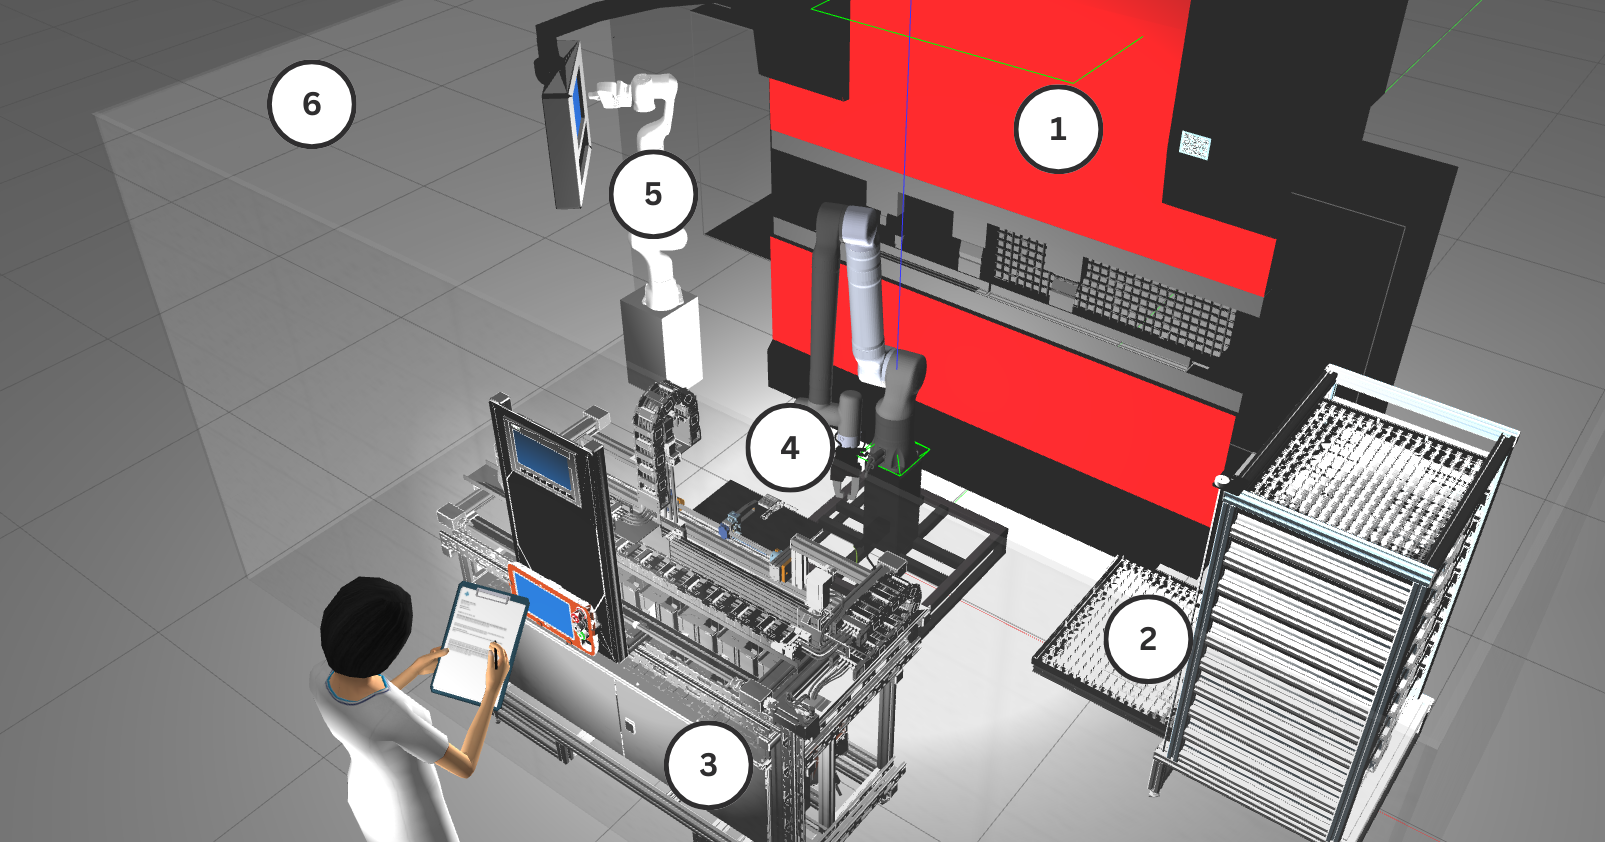
\includegraphics[width=\textwidth]{figures/robotic-workcell1.png}
    \caption{Robotic workcell layout. 1) Bending machine 2) Storage station 3) Unloading station 4) Handling robot 5) Bending machine terminal operating robot 6) Safety fence}
    \label{fig:robotic-workcell}
\end{figure}

